\documentclass[10pt,a4paper]{article}
\usepackage[utf8]{inputenc}
\usepackage[italian]{babel}
\usepackage{amsmath}
\usepackage{gensymb}
\usepackage{subfig}
\usepackage{amsfonts}
\usepackage{amssymb}
\usepackage{wrapfig}
\usepackage{graphicx}
\usepackage{xcolor}
\usepackage{float}
\usepackage{booktabs}
\usepackage[left=2cm,right=2cm,top=2cm,bottom=2cm]{geometry}
\newcommand{\rem}[1]{[\emph{#1}]}
\newcommand{\exn}{\phantom{xxx}}
\renewcommand{\thesubsection}{\thesection.\alph{subsection}}  %% use 1.a numbering
\author{Gruppo E.B24 \\ Giovanni Sucameli, Francesco Sacco, Davide Incalza}
\title{Esperienza di Fisica: Ottica I}
\begin{document}
	\date{9 Maggio 2019}
	\maketitle
    \begin{center}
		\subsection*{Introduzione}
		L'esperienza si articola in due fasi: nella prima verrà impiegato uno spettroscopio a prisma (opportunamente tarato) per la misura della lunghezza d'onda di una riga spettrale del sodio. Nella seconda verrà valutata la risoluzione di uno spettroscopio a reticolo, impiegato successivamente per la misura della costante di Rydberg sfruttando le righe di emissione dell'idrogeno.
	\end{center}


\section*{PARTE II: Misura della Costante di Rydberg}
	\subsection*{Materiale e Apparato Sperimentale}
		La seconda parte dell'esperienza impiega il seguente materiale:
		\begin{enumerate}
		    \item Spettroscopio a Reticolo
		    \item Lampada al Mercurio
		    \item Lampada al Sodio
		    \item Lampada a Idrogeno
		\end{enumerate}
	\subsection*{Calibrazione e determinazione del passo reticolare $d$}
		Come in precedenza, la stima dell'angolo zero del sistema in condizione di allineamento dei telescopi restituisce $\theta_{0} = (168.63 \pm 0.02)\degree$.
		Inizialmente occorre usare la lampada a mercurio per regolare il fuoco dello spettroscopio e misurare il passo reticolare dell'elemento dispersivo. Per questa seconda fase si pone il reticolo ad un agolo di circa 60$\degree$ e abbiamo misurato l'angolo di riflessione speculare e degli angoli rifrazione dei seguenti colori ottenendo rispettivamente:
		\begin{itemize}
		    \item Riflessione speculare $\alpha_{r} = (225.07 \pm 0.04 )\degree$, 
		    \item Frangia Viola $\alpha_{1}= (265.88\pm0.04)\degree$, $\lambda_1 = 435.833 \textrm{ nm}$
		    \item Frangia Azzurra $\alpha_{2}= (269.88\pm0.04)\degree$, $\lambda_2 = 491.068 \textrm{ nm}$
		    \item Frangia Verde $\alpha_{3} = (273.77 \pm 0.04)\degree$, $\lambda_3 = 546.074 \textrm{ nm}$
		\end{itemize}
		A seguito indicheremo $\alpha_{1},\alpha_2,\alpha_3$ con $\alpha_d$ con $d\in\{1,2,3\}$ dove $d$ sta per Diffratto.\newline
		Sfruttando le relazioni trigonometriche che legano l'angolo incidente e diffratto alle letture del goniometro:
		\begin{gather}
		    \theta_{i} = \frac{\alpha_r-\theta_0+\pi}2\\
		    \theta_{d} = \pi + \alpha_d  - \theta_0 - \theta_i
		\end{gather}
		Nell'equazione di sopra gli angoli sono misurati in radianti.
		L'equazione del reticolo impone:
		\begin{equation}
			d\cdot(\sin\theta_{i} - \sin\theta_{d}) = m\lambda_d
			\label{eq:principale}
		\end{equation}
		per cui il passo reticolare $d$\footnote{Attenzione a non confonderlo col $d$ dell'indice degli angoli $\theta_d$, la notazione è ridondante, ma combacia con quella della scheda dell'esperienza} si ottiene dagli angoli noti e dal valore di $\lambda$. Nel caso del mercurio i tre punti ricavati danno luogo ad una retta, il parametro $d$ può essere preso come parametro di \textit{fit} del modello.\newline
	    Definiamo $y_d=\sin\theta_{i} - \sin\theta_{d}$, se si considerano soltanto le diffrazioni del primo ordine $(m=1)$ è possibile determinare $d$ attraverso un fit lineare di questo tipo:
	    \begin{equation}
	    	y_d=\lambda_d/d
	    \end{equation}
	    \begin{figure}[H]
	    	\centering
		    \subfloat[Fit]{
		    \includegraphics[width=0.4\linewidth]{parte-2/immagini/passo_reticolare.eps}}\quad
		    \subfloat[Residui]
		    {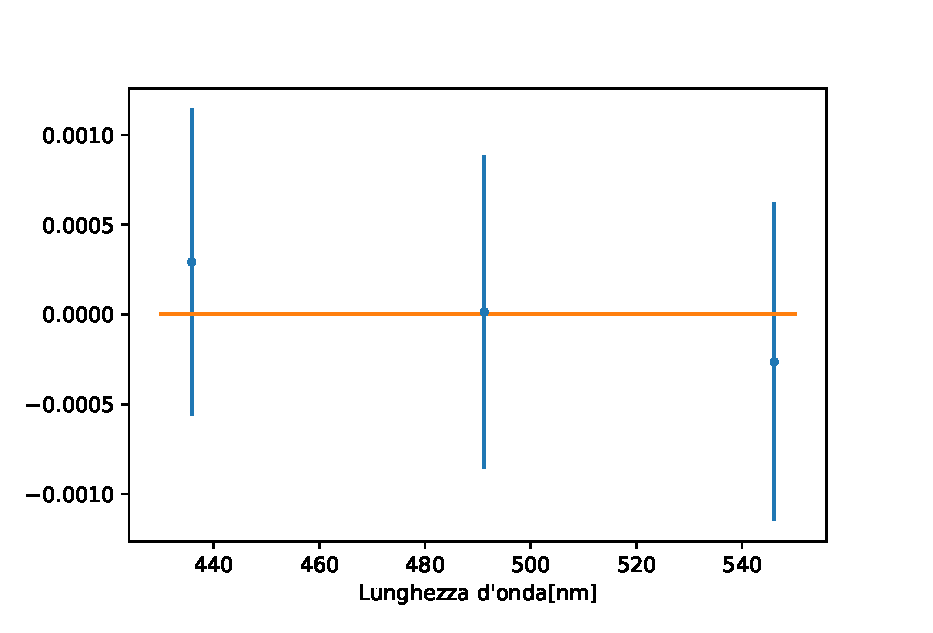
\includegraphics[width=0.4\linewidth]{parte-2/immagini/errore_passo_reticolare.eps}}
		    \caption{Fit col Mercurio per determinare il passo reticolare}
	    \end{figure}
	    l'analisi restituisce un parametro ottimale $d = 833.2\pm0.2$ nm


	\subsection*{Misura righe spettrali dell'idrogeno}
		Una volta determinata $d$ è stato possibile determinare le lunghezze d'onda dello spettro dell'idrogeno sempre con l'equazione \ref{eq:principale}.
		Facendo un pò di analisi dati le linee osservate sono:\\\\
		\begin{minipage}{.45\linewidth}
			\centering
			\includegraphics[width=\linewidth]{parte-2/immagini/idrogeno.eps}
			\captionof{figure}{Raffigurazione linee spettrali}
		\end{minipage}
		\begin{minipage}{.45\linewidth}
		\begin{tabular}{ccc}
			\hline
			Colore & $\alpha_d$ & $\lambda_d$\\
			\hline
			\begin{tabular}{ccc}
\hline
	% qua ci va il titolo della tabella (ricorda di mettere \\ alla fine) %
 \hline
	Viola & $(2.65758\pm0.00008)\times 10^{2}$ & $(4.343\pm0.002)\times 10^{2}$ \\
	Viola & $(2.65942\pm0.00008)\times 10^{2}$ & $(4.368\pm0.002)\times 10^{2}$ \\
	Azzurro & $(2.69533\pm0.00008)\times 10^{2}$ & $(4.862\pm0.002)\times 10^{2}$ \\
	Verde & $(2.73867\pm0.00008)\times 10^{2}$ & $(5.47\pm0.002)\times 10^{2}$ \\
	Verde & $(2.73942\pm0.00008)\times 10^{2}$ & $(5.48\pm0.002)\times 10^{2}$ \\
	Rosso & $(2.78725\pm0.00008)\times 10^{2}$ & $(6.164\pm0.002)\times 10^{2}$ \\
	Rosso & $(2.815\pm0.00008)\times 10^{2}$ & $(6.565\pm0.002)\times 10^{2}$ \\
	Viola II & $(2.9607\pm0.0002)\times 10^{2}$ & $(4.338\pm0.002)\times 10^{2}$ \\
	Viola II & $(2.96508\pm0.00008)\times 10^{2}$ & $(4.37\pm0.001)\times 10^{2}$ \\
	Azzurro II & $(3.03417\pm0.00008)\times 10^{2}$ & $(4.859\pm0.002)\times 10^{2}$ \\
\hline
\end{tabular}

			\hline
		\end{tabular}
		\end{minipage}
	\subsection*{Stima costante di Rydemberg}
		Secondo la teoria la lunghezza d'onda delle linee spettrali dell'idrogeno atomico sono determinate dalla seguente equazione
		\begin{equation}
			\frac1\lambda=R\bigg(\frac1{n_1^2}-\frac1{n_2^2}\bigg)
			\label{eq:ryd}
		\end{equation}
		Quest'equazione però non descrive tutte le frange dello spettro dell'idrogeno da noi osservato, ma soltanto le frequenze $434$ nm,$486$ nm,$656$ nm.\newline
		Di conseguenza abbiamo fatto un fit (figura \ref{fig:ryd}) che tiene in considerazione soltanto quelle frequenze che ci ha dato una stima della costante di Rydemberg uguale a  $(1.0972 \pm 0.0002) \times 10^{7}m^-1$ che è in linea con la previsione teorica di $1.09737$ che si trova a $0.64$ deviazioni standard dalla constante misurata.\newline
		\begin{figure}[H]
	    	\centering
		    \subfloat[Fit]{
		    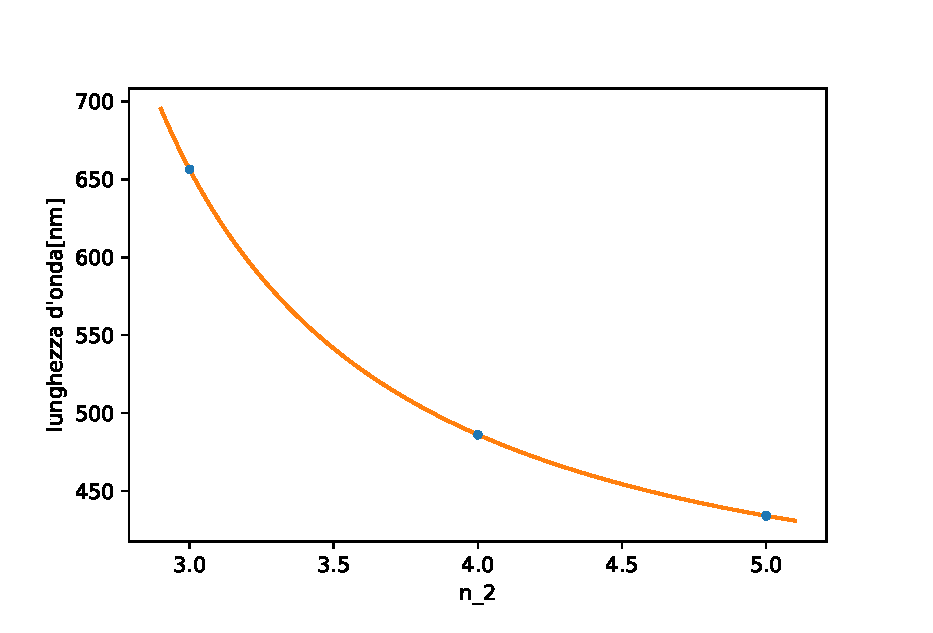
\includegraphics[width=0.4\linewidth]{parte-2/immagini/ryd.eps}}\quad
		    \subfloat[Residui]
		    {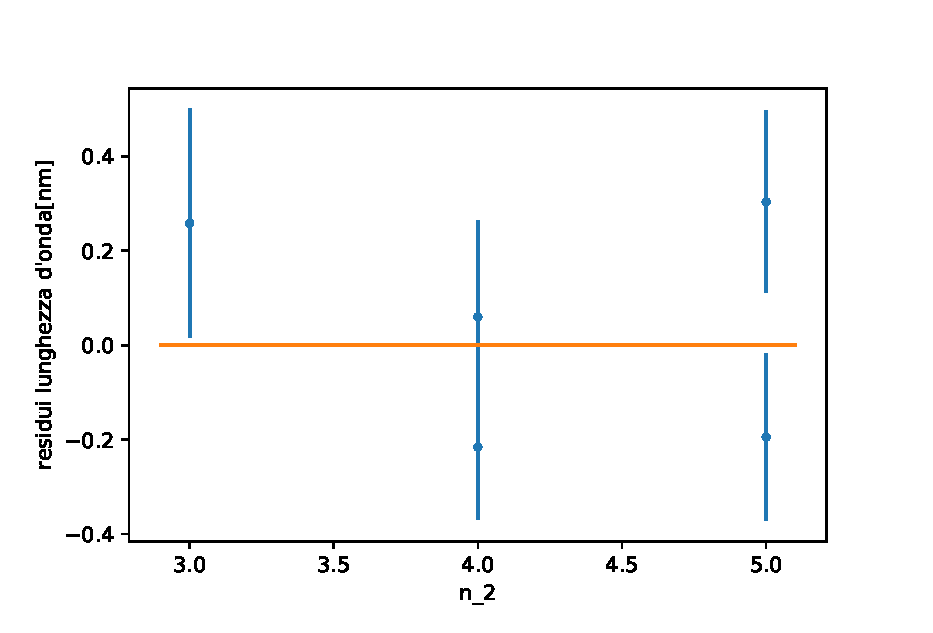
\includegraphics[width=0.4\linewidth]{parte-2/immagini/ryd_res.eps}}
		    \caption{Fit Costante di Rydemberd}
		    \label{fig:ryd}
	    \end{figure}


\end{document}